\documentclass[11pt,openright,a4paper]{report}

%%
%% Package includes to provide the basic style
%%
%%\usepackage{harvard}    % Uses harvard style referencing
\usepackage{graphicx}   % Permits import of various graphics formats
\usepackage{hyperref}   % Provides hyperlinks to sections automatically
\usepackage{pdflscape}  % Provides landscape mode for end code listings
\usepackage{multicol}   % Provides ability to split output into columns
\usepackage{listings}   % Provides styled code listings


%%
%% Set some page size changes from the standard article class
%%
\usepackage{calc}
\setlength{\parskip}{6pt}
\setlength{\parindent}{0pt}
\addtolength{\hoffset}{-0.5cm}
\addtolength{\textwidth}{2.5cm}


%%
%% Format definitions for the style
%%
%%\bibliographystyle{agsm}  %{alpha}
%%\citationstyle{dcu}
\pagestyle{headings}
\fussy


%%
%% Definitions to provide layout in the dissertation title pages
%%
\newenvironment{spaced}[1]
  {\begin{minipage}[c]{\textwidth}\vspace{#1}}
  {\end{minipage}}


\newenvironment{centrespaced}[2]
  {\begin{center}\begin{minipage}[c]{#1}\vspace{#2}}
  {\end{minipage}\end{center}}


\newcommand{\declaration}[2]{
  \thispagestyle{empty}
  \begin{spaced}{4em}
    \begin{center}
      \LARGE\textbf{#1}
    \end{center}
  \end{spaced}
  \begin{spaced}{3em}
    \begin{center}
      Submitted by: #2
    \end{center}
  \end{spaced}
  \begin{spaced}{5em}
    \section*{COPYRIGHT}

    Attention is drawn to the fact that copyright of this dissertation rests
    with its author. The Intellectual Property Rights of the products
    produced as part of the project belong to the author unless otherwise specified
    below, in accordance with the University of Bath's policy on intellectual property 
   (see http://www.bath.ac.uk/ordinances/22.pdf).

    This copy of the dissertation has been supplied on condition that anyone
    who consults it is understood to recognise that its copyright rests with its
    author and that no quotation from the dissertation and no information
    derived from it may be published without the prior written consent of
    the author.

    \section*{Declaration}
    This dissertation is submitted to the University of Bath in accordance
    with the requirements of the degree of Bachelor of Science in the
    Department of Computer Science. No portion of the work in this dissertation
    has been submitted in support of an application for any other degree
    or qualification of this or any other university or institution of learning.
    Except where specifically acknowledged, it is the work of the author.
  \end{spaced}

  \begin{spaced}{5em}
    Signed:
  \end{spaced}
  }


\newcommand{\consultation}[1]{%
\thispagestyle{empty}
\begin{centrespaced}{0.8\textwidth}{0.4\textheight}
\ifnum #1 = 0
This dissertation may be made available for consultation within the
University Library and may be photocopied or lent to other libraries
for the purposes of consultation.
\else
This dissertation may not be consulted, photocopied or lent to other
libraries without the permission of the author for #1 
\ifnum #1 = 1
year
\else
years
\fi
from the date of submission of the dissertation.
\fi
\vspace{4em}

Signed:
\end{centrespaced}
}

%%
%% END OF DEFINITIONS
%%

    %% These are the includes required for the doc 

\usepackage{hyperref}
\usepackage[parfill]{parskip}
\usepackage{csquotes}
\usepackage{graphicx}
\usepackage[toc, page]{appendix}
\usepackage[
  backend=bibtex,
  style=authoryear,
  citestyle=authoryear,
  dateabbrev=false
]{biblatex}

% Number enumerate sub enumerates
\renewcommand{\labelenumii}{\theenumii}
\renewcommand{\theenumii}{\theenumi.\arabic{enumii}.}

% Biblatex long urls fix
\makeatletter
\def\blx@maxline{77}
\makeatother

% Fix to apply hyperref to whole biblatex citation instead of just year.
\DeclareCiteCommand{\parencite}[\mkbibparens]
  {\usebibmacro{prenote}}
  {\usebibmacro{citeindex}%
    \printtext[bibhyperref]{\usebibmacro{cite}}}
  {\multicitedelim}
  {\usebibmacro{postnote}}

\DeclareCiteCommand*{\parencite}[\mkbibparens]
  {\usebibmacro{prenote}}
  {\usebibmacro{citeindex}%
    \printtext[bibhyperref]{\usebibmacro{citeyear}}}
  {\multicitedelim}
  {\usebibmacro{postnote}}
% End biblatex fix

\title{Development of an extensible personal informatics system to aid in self management of mental health and wellbeing, making use of both user provided data and user specific API data}
\author{Liam Crewe}
\date{Bachelor of Science in Computer Science with Honours\\University of Bath\\May 2017}

\addbibresource{bibtex.bib} 

\begin{document}

% Set this to the language you want to use in your code listings (if any)
\lstset{language=Java,breaklines,breakatwhitespace,basicstyle=\small}

\setcounter{page}{0}
\pagenumbering{roman}

\maketitle
\newpage


% Set this to the number of years consultation prohibition, or 0 if no limit
\consultation{0}
\newpage


\declaration{Development of an extensible personal informatics system to aid in self management of mental health and wellbeing, making use of both user provided data and user specific API data}{Liam Crewe}
\newpage


\abstract
Your abstract should appear here.  An abstract is a short
paragraph describing the aims of the project, what was
achieved and what contributions it has made.
\newpage


\tableofcontents
\newpage
\listoffigures
\newpage
\listoftables
\newpage


\chapter*{Acknowledgements}
Add any acknowledgements here.
\newpage


\setcounter{page}{1}
\pagenumbering{arabic}

\chapter{Introduction}
\section{Background}
\subsection{Mental Health in the UK}
One in four adults (around 26\%) have been diagnosed with at least one mental health condition \parencite{hse2014} (where adult is any person 16 or over). A further 18\% reported to have experienced a mental health condition but did not seek a diagnosis \parencite{hse2014}. This equates to around 44\% of adults in the UK. The population of the UK is around 65 million \parencite{onspopulation}, of which around 18.8\% are under the age of 16 \parencite{onspopulation}. This equates to a population over the age of 16 of around 81.2\%, or around 52.78 million people. Given that 44\% of these will experience a mental health condition, this equates to over 23 million adults in the UK alone suffering from mental health conditions. This, in addition to any children and young people with mental health conditions truly shows the prevalence of mental health conditions in the UK.

This figure is further supported by the fact that mental health is the result of over 70 million sick days every year \parencite{cmoreport2013}, and is the largest burden of disease with around 28\% of the total burden, compared to 16\% for each of cancer and heart disease \parencite{burdendisorders}. Mental health conditions are estimated to cost the economy between £70 and £100 billion every year \parencite{cmoreport2013}.

\subsection{Mental Health Funding and Capacity}
Despite these figures, the funding for mental health services only sums to around 13\% of total NHS spending \parencite{cepnhsfunding}. In fact, around 75\% of people with mental health conditions receive no treatment at all \parencite{cmoreport2013}. On top of this, although the NHS (National Health Service) is due to receive increased funding in 2016 and the years that follow \parencite{kfnhsbudget}, funding for mental health services is due to rise by just 0.3\% \parencite{mhfunding}. 53 out of 59 services in the UK responded to the freedom of information act made as part of the cited BBC article by \citeauthor{mhfunding}; 23 of which said that their funding would in fact decrease in 2016.

\section{Problem Description}
\subsection{Self Management in Mental Health}
This project is not aiming to find a way to increase the supply of treatment from mental health services, but rather to reduce the demand for it. Much research has been done into the effectiveness of self management for mental health conditions. For example, a study in 2011 tested a particular self management scheme and found that it \enquote{reduces psychiatric symptoms, enhances participants’ hopefulness, and improves their QOL over time} \parencite{wrapstudy}. This shift to self management could help ease the pressure on mental health services, by relieving some of the demand and allowing users to manage their conditions before they worsen. It has also proven particularly effective for relapse prevention in people who have previously undergone treatment for mental health conditions, in that it has been described to \enquote{play a critical role in people's recovery from mental illness} \parencite{selfmanagementrelapse}.

\subsection{Personal Informatics in Mental Health}
This relates to a field known as personal informatics. \enquote{Personal informatics is a class of tools that help people collect personally relevant information for the purpose of self-reflection and self-monitoring} \parencite{personalinformatics}. Personal informatics in mental health is an interesting topic. In 2011 a project aimed to create a personal informatics system that combined sensor data with user inputted data, with the aim of allowing self management of bipolar disorder \parencite{pimentalhealth}. This study found that although personal informatics systems had clear relevance to mental health treatment, little research had been done in the area. It also concluded that the if a system could fuse the collection of personal data into treatment tools in some way, this may have relevance to other mental health disorders, as well as more mild issues such as stress management and the building of balanced, productive lifestyles.

Various applications already exist to allow self management of mental health conditions, such as Optimism \parencite{optimism}. This works by collecting user inputted data and building visualisations the user can look at and draw conclusions from.

While this method of user inputted data works, it is flawed for several reasons. Firstly, users may not be aware of what is a dangerous pattern \parencite{pimentalhealth}, and secondly it requires users to fill in (sometimes lots of) fields fairly frequently. This could lead users to not use the system as often as they could and should. This could be avoided; many modern applications already record data about users, either via user input or automatically. There are many examples of these: mental health apps such as Optimism \parencite{optimism}, fitness apps such as Strava \parencite{strava}, social media apps such as Twitter \parencite{twitter} and many others. This results in a huge amount of data being recorded and made available from applications the user may already use, without requiring the user to submit the data themselves.

This data is very important to this project as mental health is affected by such a wide variety of factors. The examples above for example are discussed below:

\subsubsection{Exercise}
It is common to recommend exercise as a way to help with various mental health conditions. Physical activity is known to alleviate symptoms of mild to moderate depression and has been associated with improvement of self-concept and confidence, as well as reduced symptoms of anxiety \parencite{exercisementalhealth}. Various apps such as Strava \parencite{strava} track how much and how often a user exercises, and could allow the user to correlate exercise frequency and duration with mental health issues.

\subsubsection{Social Media}
It has been shown for example that Facebook can cause depression in some teens when used excessively \parencite{fbdepressionteens}. A research team at Microsoft was even able to build a classifier that used Twitter data to predict onset depressive episodes in patients with major depression, with an accuracy of around 70\% \parencite{de2013predicting}.

\subsection{This Project}
\subsubsection{Overview}
This project aims to take advantage of this data by producing an application called SelfReflect. SelfReflect will only require the user to record a small amount of data about themselves. This will consist of a simple wellbeing questionnaire, which will calculate a wellbeing score. This will then be recorded, along with date and time of submission. The exact nature of this questionnaire will be discussed later, but the key part is that the questionnaire produces a reliable mental health wellbeing score, and is simple, fast and easy for the user to fill out, with the goal that this will allow the user to record their wellbeing more often.

SelfReflect will consist of three distinct parts: a mobile app to allow recording of wellbeing (and automatically date and time of submission), a server side application programming interface (API) to allow storing and retrieval of user data and a web app. The web app will allow the user to add credentials (via the SelfReflect API) to various apps such as Twitter and Strava. This will allow SelfReflect to pull data from these apps via their individual APIs. The web app will then allow the user to interrogate this data and produce visualisations across the multiple data sources.

The goal of this is not to produce a system with an extensive variety of sources and visualisations for the user. Entire projects could be completed on producing lots of different visualisations from just one of these sources with regard to mental health. Instead, SelfReflect will be developed to be extensible; to be built on in the future. Support for two sources (Twitter and Strava) will be developed, with one visualisation for each, as \enquote{proofs of concept}, but this is by no means the final goal of the software system. The API will be built in such a way that a user (or developer) can fetch their data from each source via the SelfReflect API (given that they have provided valid credentials), providing an \enquote{API of APIs}. Also, the API will return \emph{all} data it can access for the user from that source, rather than having one endpoint per visualisation, allowing multiple visualisations to be built from each source in the future.

\section{Aims} \label{aims}
\begin{itemize}
\item Design a system to aid self management of mental health by combining user submitted data with existing applications data., and producing visualisations from this combined data.
\item Design this system to be extensible, so that it can be built on in the future via the addition of more options for sources, more visualisations for new and/or existing sources.
\item Test this system in both a functional and user experience context, including the usability of the various aspects of the system.
\item Investigate the feasibility of this tool as an aid for self management of mental health.
\end{itemize}

\section{Objectives} \label{objectives}
\begin{itemize}

\item Design and implement an API that allows:
\begin{itemize}
  \item User creation, log in and management.
  \item Storage of wellbeing score, as well as date and time of submission.
  \item Fetching of user's wellbeing scores over time.
  \item Connection of existing applications (Twitter and Strava) when given valid applications credentials for a user, and storage of these credentials.
  \item Fetching of user's existing application data, to create an \enquote{API of APIs}
\end{itemize} 
  
\item Design and implement a mobile app that allows:
\begin{itemize}
  \item User creation and log in.
  \item Recording of wellbeing score, as well as date and time of submission.
\end{itemize}

\item Design and implement a web application that, via the API disscussed above, allows:
\begin{itemize}
  \item User creation, log in and management.
  \item Recording of wellbeing score, as well as date and time of submission.
  \item Connection of existing applications when given valid applications credentials for a user.
  \item Fetching and combining of user's data from both SelfReflect and connected existing applications, to produce visualisations from this data (one for each of the \enquote{proof of concept} sources.
  \item 
\end{itemize} 

\item Distribute this application to a series of volunteer testers, and get feedback on both the functionality of the system (i.e. if it works) and the usability of the various areas of the system.
\item Analyse the application and the results of the testing to:
\begin{itemize}
  \item Identify possible future changes that could be made and functionality/features that could be added in order to improve the system.
  \item Identify the effectiveness of the sources and visualisations system, and improvements that can be made to it.
  \item Discuss the extensibility of this application for future development.
  \item Discuss the feasibility of this application as a tool for self management of mental health.
\end{itemize}

\end{itemize}

%%%%%%%%%% @TODO:
%% May need to update this later. Depends what goes in each section.
\section{Dissertation Structure}
\textbf{Chapter 1: Introduction}

This chapter provides some high-level background research and motivation for the project, and gives an overview of the project, including its aims and objectives.

\textbf{Chapter 2: Literature Survey}

This chapter delves deeper into the research relevant to this project. It considers relevant literature in terms of motivations and system design, researches methods of recording wellbeing, and compares and contrasts existing applications.

\textbf{Chapter 3: Requirements Specification}

This chapter details the functional and non functional requirements for the system, as derived from the project aims and objectives, and the literature survey. It also discusses the gathering, development and terminology of these requirements.

\textbf{Chapter 4: Design}

This chapter details the design of the three parts of the system (API, mobile app and web app), in order to fulfil the requirements as defined in chapter 3.

\textbf{Chapter 5: Implementation}

This chapter details the implementation of the design as defined in chapter 4.

\textbf{Chapter 6: Testing}

This chapter first discussed automated testing, then continues to detail the methods used for testing functionality, usability and feasibility of the system, using volunteer testers.

\textbf{Chapter 7: Results and Discussion}

This chapter presents the results of the testing by the volunteer testers. It then discusses these results, improvements that could be made to the system based on these results, and the feasibility of the system as a tool to aid in self management of mental health and wellbeing.

\textbf{Chapter 8: Conclusion and Future Work}

This chapter summarises the project and discusses its successes and failures. It also details areas for improvement and for future work.

%%%%%%%%%%

\chapter{Literature Survey} \label{litsurvey}
\section{Introduction} \label{introduction}
This literature survey will identify the various fields this project relates to. It will then present and critique existing work related to these fields, both in the form of academic research and existing technologies. By doing so, it will discuss what exactly this project hopes to contribute to these fields, how it plans to do so, and how this contribution would be useful.

This project encompasses two key fields: personal informatics and mental health. These are two active areas of research, as will be shown and discussed in later sections. This project hopes to combine these two fields in ways that will contribute to them, both in an academic sense, and with the development of a software system that encompasses both of these fields, to aid people in the effective self management of their mental health and wellbeing.

The existing research in these fields will be extremely useful in the design and development of the system and its requirements. These will be developed by drawing on the conclusions of existing work, and by making improvements on existing technologies.

\subsection{Self Management in Mental Health}
Self-management techniques and schemes have been shown to be effective in both treatment \parencite{wrapstudy} and recovery \parencite{selfmanagementrelapse}. Many schemes exist today and are growing in popularity, with these schemes being said to offer an \enquote{increasingly popular alternative to therapist-administered psychological therapies, offering the potential of increased access to cost-effective treatment} \parencite{selfhelpanxiety}.

Much of the principle of self-management revolves around \enquote{empowerment} of the user \parencite{whoselfmanagement}. Empowerment involves the user in decisions about his or her mental health condition treatment, providing them with a level of control and influence \parencite{whoempowerment}. Although self-management and active engagement has been commonplace for physical long term health conditions for a long time, it has been much less widely used in the context of mental health \parencite{whoselfmanagement}. It is only fairly recently that this has become common in mental health treatment, with claims that it can be as effective as medical treatment \parencite{mhfselfmanagement}.

For a long time, mental health patients were thought of as passive recipients of care, but attitudes have changed over recent years \parencite{cpselfmanagement}. It was discovered that empowering users significantly improved treatment and recovery, giving users the \enquote{knowledge, skills, and self-confidence} to \enquote{take care of their own health and manage to live life competently} \parencite{vahdatpatientinvolvement}.

Many self-management schemes are based around teaching users specific skills, and providing them with the tools and techniques required to manage their mental health by themselves \parencite{selfmanagementuk}. The amount of clinical intervention required varies depending on the scheme, ranging from pure self help techniques (no clinical involvement) to guided self help (some clinical involvement), be that through face-to-face sessions, telephone or email \parencite{selfhelpanxiety}.

There are lots of self-management techniques, many of which are common recommendations to those suffering from mental health conditions or poor mental health. Some of these common techniques will be discussed below, with regard to how they apply to this project, and how this project can aid execution of each technique.

\subsubsection{Cognitive Behavioural Therapy (CBT) Techniques}
Cognitive Behavioural Therapy, or CBT, is a form of talking therapy that is extremely popular in modern mental health treatment. It is \enquote{one of the most extensively researched forms of psychotherapy}, which is \enquote{due in part to the ongoing adaptation of CBT for an increasingly
wider range of disorders and problems} \parencite{butler2006empirical}.

Although CBT itself is not a self-management technique, it involves users learning mental health management tools, known as CBT techniques, that can be used in daily life after treatment ends \parencite{babcpcbt}. CBT works by changing how a person interprets or reacts to things that happen to or around them, and teaching them to identify harmful, negative or unbalanced reactions \parencite{nhscbt}. This is in itself a self-management technique, and has been said to be one of the main reasons CBT has such impressively low relapse rates. A study by \citeauthor{butler2006empirical} (\citeyear{butler2006empirical}) revealed that for patients treated for depression, on average \enquote{only 29.5\% of CBT patients relapsed versus 60\% of patients treated with antidepressants}.

CBT is a combination of two types of therapy: cognitive and behavioural \parencite{patientcbt}. Cognitive techniques relate to negative thoughts, and to what a person thinks, or how a person reacts emotionally to a situation or event \parencite{medscapecbt}. It is be unlikely that the system developed in the project will be able to directly measure the effectiveness of cognitive techniques.

Behavioural techniques however often involves substituting alternate, less harmful behaviours for harmful ones \parencite{patientcbt}. If this behaviour is one measured by a system, such as exercise or social activity, its effectiveness could be measured by the system and reported to the user. This could allow the user to identify which CBT techniques are more useful to them, as well as the effect on their mental health of not employing these techniques. They could also identify when a technique or techniques become less effective, and either address this themselves or recognise this as a sign of relapse, and consider contacting a mental health clinician before their condition worsens.

\subsubsection{Trigger Identification}
Triggers refer to events that can potentially result in relapses or negative impacts on mental health \parencite{samhsatriggers}. These events can \enquote{trigger} these issues. Users identify triggers and plan their responses in advance so that they can react appropriately to try to avoid negative consequences \parencite{samhsatriggers}.

The aim of this system in regard to triggers is that, should a user experience a negative change in mood, they can view the data around that time and identify potential triggers that resulted in that negative change. They can also, in a similar way to CBT techniques, measure the effectiveness of their planned actions to triggers. If the user knows a trigger occurred, and a planned action was carried out, they can investigate how effective this reaction was in avoiding the negative consequences of the trigger.

\subsubsection{Wellness Recovery Action Plan (WRAP)}
Wellness Recovery Action Plan, or WRAP, is another popular and widely used system for self-management \parencite{mhrwrap}. There is some crossover with the above methods. A user creates their own WRAP, which includes (definitions taken from \parencite{mhrwrap}):
\begin{itemize}
\item A \enquote{Wellness Toolbox}. That is, resources such as contacting friends, exercising and maintaining a healthy diet.
\item A daily maintenance plan; tasks to do every day to maintain wellness.
\item Triggers; as discussed above.
\item Early warning signs of worsening symptoms.
\item A plan for when things are breaking down, or when things are getting much worse.
\item A crisis plan; signs that inform others your care needs to be taken over, and what they should do.
\item A post crisis plan; what to do to get yourself well again.
\end{itemize}

This clearly has some crossover with the above methods. Again, the system developed in this project would in theory be able to help with this. An early warning sign, or even later sign could be identified by the wellbeing data recorded in the system. The effectiveness of the daily maintenance plan and post crisis plan could also be measured, and potentially updated depending on the results of the data recorded. This also applies to the Wellness Toolbox.

\subsubsection{Self Management Schemes Similarities}
All three of these schemes have some common features. They all require:
\begin{itemize}
\item Identification/recognition of events that can cause negative consequences to mental health.
\item Recognition of when these events happen and the effect of them.
\item Planned actions to minimise/counteract the negative consequences of these events.
\end{itemize}

To do this, and to measure the effectiveness of these actions, some measurement of mental wellbeing needs to be made regularly. In theory, this would be best if made both before and after the trigger, as well as after the planned action (or a while after the trigger if no planned action is taken).

This is particularly important for the purposes of this system. Only if this measurement is effective, efficient and recorded regularly will the system be able to aid in these self-management techniques. This is another area that requires research and a review of existing work, in order to decide the best way to allow the user to record their wellbeing easily and effectively.

\subsection{Recording of Mental Health and Wellbeing} \label{recordingmentalhealth}
\subsubsection{Method of Recording} \label{methodofrecording}
There are two key ways to record a person's wellbeing: self-rating and observer rating. For the purposes of this project, self-rating will be used, as the application is designed for self-management. Regardless of the fact that this is necessary for this project, self-rating methods may well be more effective anyway. A study in 2011, published in the journal of mental health, investigated the effectiveness of various measures from the point of view of service users \parencite{crawford2011selecting}.

This study highlighted the importance service users place on measures rated by the patient. The participants in the study even \enquote{expressed surprise, and in some instances disbelief, that outcome measures based entirely on the judgements of researchers or clinicians could be used to judge a person’s response to treatment}. This study will be particular useful when discussing how to record mental health and wellbeing.

\subsubsection{Ecological Momentary Assessment (EMA)} \label{sec:ema}
Ecological momentary assessment (EMA) refers to a method of data collection in which a person can \enquote{report on symptoms, affect and behaviour close in time to experience} \parencite{moskowitz2006ecological}. This strongly relates to this project, as a key aim is to allow users to record their wellbeing regularly and easily, allowing EMA. EMA has \enquote{a number of advantages over more traditional methods for the assessment of patients}, and has been shown to \enquote{permit more sensitive assessments} and \enquote{enable more wide-ranging and detailed measurements of mood and behaviour} \parencite{moskowitz2006ecological}.

\subsubsection{Questionnaire Length and Response Burden} \label{questionnairelength}
Another important consideration is the length of the method used to record wellbeing. This relates to a concept known as \enquote{response burden}. That is, the effort required by a user to answer a questionnaire \parencite{rolstad2011response}. The initial proposal for this project was for the questionnaire length to be just one field, rating a mood or wellbeing on a simple scale. However, research shows that users accused questionnaires that are too short of not being able to \enquote{properly assess the complex
outcomes they are designed to measure} \parencite{crawford2011selecting}.

Questionnaires that are too long however have been shown to result in a lower response rate, and faster, shorter, more uniform responses to later questions \parencite{galesic2009effects}. This is possibly due to the questionnaire having too large a response burden for the user. The user may become bored or disillusioned with the measure and think less about responses.

A high response burden poses another problem for this project, in that this system aims to allow users to record their wellbeing quickly and easily. A higher response burden could lead to the user delaying the recording of their wellbeing, which would then not count as EMA. To overcome this, the system must implement some trade off between response burden, and obtaining meaningful measures of mental health and wellbeing.

\subsubsection{Outcome Measures}
In both mental and physical health, measurements of a patient's progress and the efficacy of their treatment are often referred to as \enquote{outcome measures} \parencite{pediaoutcomemeasures}. These measures are said to allow health services to improve quality of service, but can also be used in the context of tracking a patient's mental health and wellbeing. These measures come in many forms, and fall into various possible categories: general outcome measures, patient rated outcome measures (PROMS), outcome measures for use with children, outcome measures for emotional difficulties and various others \parencite{mhpoutcomemeasures}. As discussed in section \ref{methodofrecording} above, we are only interested in self-rating methods, and hence will only investigate patient reported outcome measures.

\subsection{Which Outcome Measure(s)?} \label{whichoutcomemeasures}
There are many condition specific outcome measures, for example the \enquote{Patient Health Questionnaire} (PHQ-9) for depression \parencite{kroenke2001phq}, and the \enquote{Generalized Anxiety Disorder} (GAD7) questionnaire for generalised anxiety disorder \parencite{spitzer2006brief}.

These condition specific questionnaires may well be more effective than generic wellbeing questionnaires. This project however will focus on the more generic examples. This is due to the fact that the key goal of this project is to investigate the combinations of user provided wellbeing data with user specific API data. The scope of the project does not allow for investigation and development of a new or custom outcome measure. Neither does it allow for the inclusion of multiple condition specific outcome measures. A key goal of the application is that it is generic, and at least somewhat applicable to the majority of the general population, in regards to keeping track of their mental health and wellbeing.

For these reasons the project will implement an existing, well established patient reported outcome measure. Some examples of existing, popular outcome measures will be discussed, as will their appropriateness for use in this project. Candidates to be discussed (one of which will be included in the system) are: the \enquote{European Quality of Life instrument} (EQ-5D), the \enquote{Recovery Star}, the \enquote{Warwick-Edinburgh Mental Wellbeing Scale} (WEMWBS), and its short version, the \enquote{Short WEMWBS} (SWEMWBS).

\newpage
\subsubsection{European Quality of Life instrument (EQ-5D)}
The \enquote{European Quality of Life instrument} (EQ-5D) is a \enquote{standardized instrument for use as a measure of health outcome} \parencite{eq5dabout}. The questionnaire consists of two pages. The user answers 5 questions on a scale from \enquote{no problem} to \enquote{unable to do} in areas such as mobility and self care, then scores their mood on a scale of 1 to 100 \parencite{eq5duse}. An example EQ-5D can be seen in Figure \ref{fig:eq5d} (images from \parencite{eq5duse}):

\begin{figure}[ht]
\caption{The European Quality of Life Instrument}
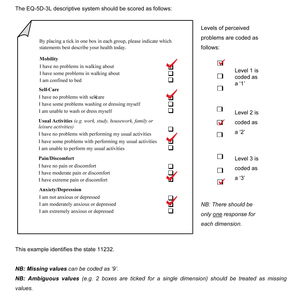
\includegraphics[width=.5\textwidth]{i/eq5d1.jpg}\hfill
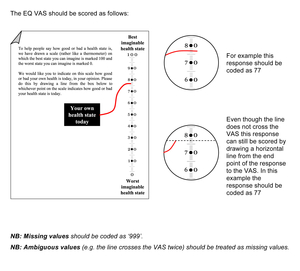
\includegraphics[width=.5\textwidth]{i/eq5d2.jpg}
\label{fig:eq5d}
\end{figure}

The EQ-5D has been shown to be useful for common mental health conditions such as mild to moderate depression \parencite{brazier2010eq}, which may well be appropriate for this system. However, it is possible it suffers from an issue discussed in the section \ref{questionnairelength} above; it is too short. In fact, in the study by \citeauthor{crawford2011selecting}, it was this questionnaire that participants raised concerns about with regard to it being too short to properly assess complex outcomes \parencite{crawford2011selecting}.

\newpage
\subsubsection{Mental Health Recovery Star (MHRS)}
The \enquote{Mental Health Recovery Star} (MHRS) is part of a set of outcome measure tools called \enquote{Outcomes Stars} \parencite{outcomesstars}. It measures ten areas of a user's life, rating them on a scale of 1 to 10, where 1 is \enquote{stuck} and 10 is \enquote{self-reliance}. This then produces a graphic in the shape of a ten-pointed star, an example of which can be seen in Figure \ref{fig:mhrs} (image from \parencite{outcomesstars}):

\begin{figure}[ht]
\centering
\caption{The Mental Health Recovery Star}
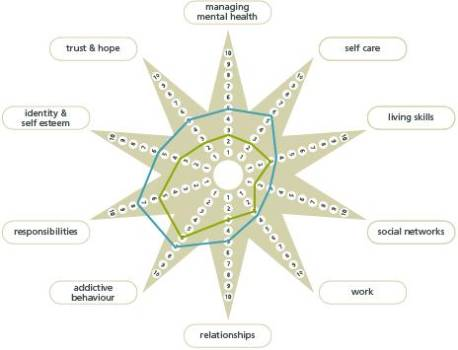
\includegraphics[width=\textwidth]{i/recoverystar.jpg}]
\label{fig:mhrs}
\end{figure}

This measure has been \enquote{received enthusiastically by both
mental health service providers and service users} \parencite{dickens2012recovery}. A study by \citeauthor{killaspy2012psychometric} aimed to analyse the psychometric properties of the MHRS \parencite{killaspy2012psychometric}. It found some positive results, revealing that 85\% of participants found the MHRS useful in areas such as planning support and tracking their recovery. It also found that 70\% of participants said the MHRS was easy to use. However, this study only considered MHRS recorded either by staff or collaboratively with staff and user.

Staff or collaborative recording is common with the MHRS; many staff are given training in order to guide users in using the measure. In fact, training is now a requirement to gain a license to use the star \parencite{starlicense}. Clearly this poses an issue for this project. Assuming a license could be obtained without training (which may be unlikely), it is possible that this training issue could be overcome with computerised tutorials and careful user experience design. However, this would still require the user to learn how to use the MHRS, and would be more complicated than a more simple, intuitive outcome measure.

Another issue with MHRS is the time to complete. In the study by \citeauthor{killaspy2012psychometric} it was found that it, on average, took 30 to 60 minutes to complete \parencite{killaspy2012psychometric}. While this was posed as a positive in this study, it is likely a negative for the purposes of this project. Response burden needs to be considered with regard to the desired frequency of response. For this project, the aim is to have a high frequency of response, meaning users will be able to regularly record their wellbeing. This could be multiple times per week, once per day or even multiple times per day. 

When considering 30 to 60 minutes with regard to this high desired response frequency, this is quite a high response burden. As discussed in the questionnaire length and response burden section, this is a key problem for this project. Also, it is likely that this time will be even longer than 30 to 60 minutes, given that the user would be completing the MHRS on their own without the guidance of a trained member of staff.

\subsubsection{Warwick-Edinburgh Mental Wellbeing Scale (WEMWBS)}
The \enquote{Warwick-Edinburgh Mental Wellbeing Scale} (WEMWBS) is a scale designed to \enquote{enable the monitoring of mental wellbeing in the general population} \parencite{wemwbs}. It was developed by a panel of experts \parencite{wemwbsdevelopment} and has been tested fairly extensively, finding that it \enquote{showed good content validity} and is a \enquote{short and psychometrically robust scale} \parencite{tennant2007warwick}. It consists of 14 positively worded items with 5 possible responses to each, ranging from \enquote{none of the time} to \enquote{all of the time}.
\newpage
These questions and responses can be seen in Figure \ref{fig:wemwbs} (table from \parencite{wemwbsquestions}):
\begin{figure}[ht]
\centering
\caption{The Warwick-Edinburgh Mental Wellbeing Scale}
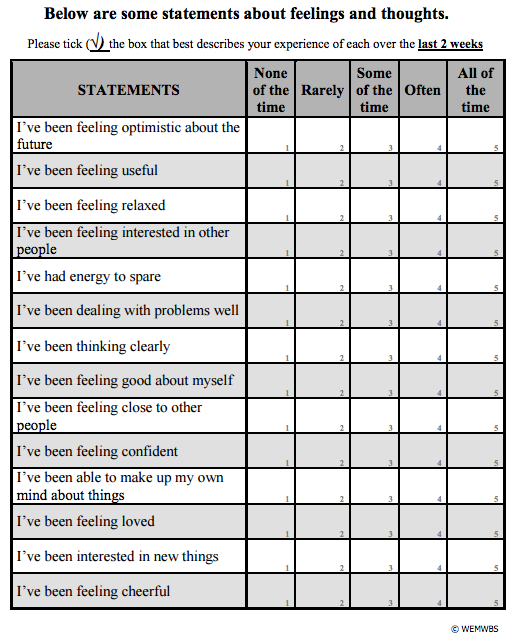
\includegraphics[width=.8\textwidth]{i/wemwbs.png}
\label{fig:wemwbs}
\end{figure}

The fact that WEMWBS was developed for the general population is particular useful to this project, as a general purpose, simple scale is exactly what this project requires. Another strength of this scale is that it results in a single score, which is simply a sum of the responses. Each response is scored 1-5, giving a score of 14-70 for the full questionnaire \parencite{wemwbsscoring}. This is beneficial to this project as a single score can be easily recorded and mapped against other data such as date/time, or user specific API data such as social media activity.

The study by \citeauthor{crawford2011selecting} found the WEMWBS to be largely successful, in that it achieved one of the highest ratings among participants \parencite{crawford2011selecting}. This study identified another key problem with various outcome measures. This was the use of negatively phrased questions, as users said it can be \enquote{upsetting to be asked long lists of questions about difficulties associated with mental ill
health}. The WEMWBS was commended by participants for phrasing items positively, where poor mental health would be recognised by a lack of these positive terms, rather than the presence of negative terms.

A problem with WEMWBS however is the length of the questionnaire, in that it consists of 14 items. This shouldn't be too time consuming for the user as the questions are not open ended, and are relatively simple. However, again regarding the aim of a high response frequency, a shorter questionnaire may be more effective for the purposes of this project. Thankfully, a shorter version of the WEMWBS exists; the \enquote{Short WEMWBS} (SWEMWBS).

\subsubsection{Short WEMWBS (SWEMWBS)} \label{swemwbssection}
The \enquote{Short WEMWBS} (SWEMWBS) is a shorter version of the WEMWBS, consisting of a 7 item scale rather than a 14 item scale \parencite{swemwbs}. The questions on the short version are a subset of those on the full version, so retain the advantages of being positively worded. In order to compare the two scales, the score obtained from the shorter version is mapped to an equivalent longer version score via a conversion table. This conversion table can be seen in appendix \ref{swemwbsconversiontable}.
\newpage
The questions in the SWEMWBS can be seen in Figure \ref{fig:swemwbs} (table from \parencite{swemwbsquestions}):
\begin{figure}[ht]
\centering
\caption{The Short Warwick-Edinburgh Mental Wellbeing Scale}
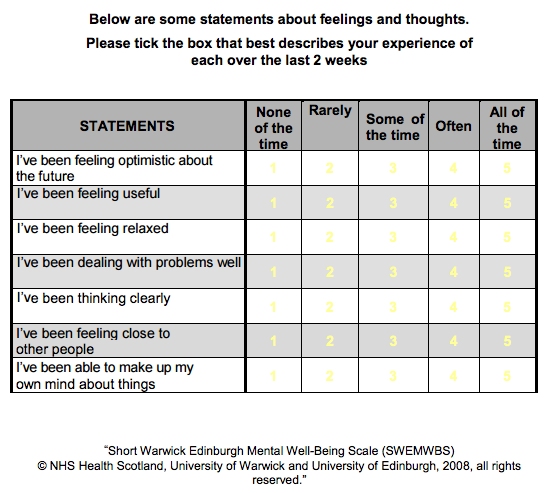
\includegraphics[width=.8\textwidth]{i/swemwbs.png}
\label{fig:swemwbs}
\end{figure}

The scale was developed in a research project by \citeauthor{stewart2009internal} (\citeyear{stewart2009internal}). This project tested the shorter scale and drew various conclusions on its validity and effectiveness. While the longer version of course provides more detail, the r-value was found to be 0.954 in the development and testing of the scale, meaning the scores produced are very similar. Given the high correlation of scores, the lower response burden and robust measurement properties of SWEMWBS, this testing found that this made \enquote{SWEMWBS preferable to WEMWBS at present for monitoring mental wellbeing in populations} \parencite{stewart2009internal}.

The disadvantages of this scale are that, as discussed, it does provide a more narrow view of a person's wellbeing. \citeauthor{stewart2009internal} (\citeyear{stewart2009internal}) found that where \enquote{face validity is an issue there remain arguments for continuing to collect data on the full 14 item WEMWBS}. However, for the purposes of this project a simpler scale with lower face validity is preferable.

The SWEMWBS (as well as the WEMWBS) is copyrighted by the University of Warwick and NHS Health Scotland. However, it is free to use as long as users register by completing a registration form \parencite{wemwbsreg}.

\subsubsection{This project}
The SWEMWBS will be used for this project as it seems to provide a good trade off between response burden and obtaining meaningful measures of mental health and wellbeing. It is publicly available (after registration) and provides a single wellbeing score per response, which will aid massively when building visualisations. This will make mapping of wellbeing to other factors simple, which should result in simple, effective and easy to understand visualisations for the user.

\section{Personal Informatics} \label{personalinformatics}
\subsection{Introduction}
Personal informatics can be defined as software that is designed to \enquote{help individuals collect personal information to improve self-understanding}, allowing them to \enquote{promote positive behaviors} such as \enquote{healthy living, energy conservation, etc.} \parencite{li2012personal}.

\subsection{Stages of Personal Informatics}
A study by \citeauthor{li2010stage} developed a 5 stage model to represent personal informatics systems, consisting of \enquote{preparation, collection, integration, reflection, and action} \parencite{li2010stage}.
\newpage

This study produced a diagrammatic representation of these stages, which is shown in Figure \ref{fig:5stagespi}.
\begin{figure}[ht]
\centering
\caption{Five Stage Model of Personal Informatics}
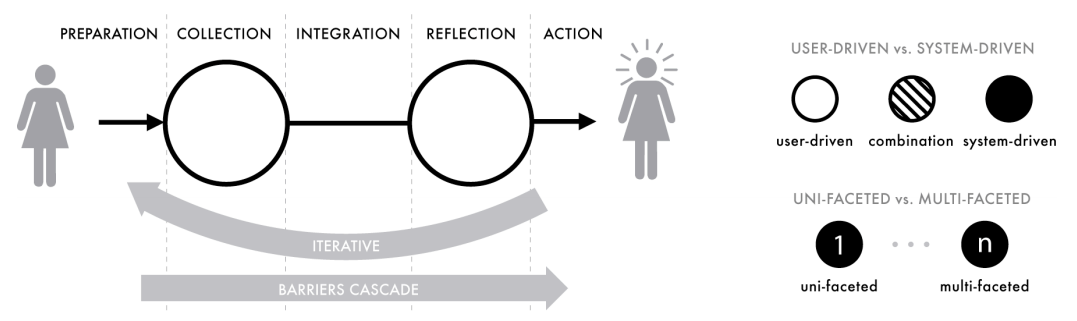
\includegraphics[width=\textwidth]{i/5stagespi.png}
\label{fig:5stagespi}
\end{figure}

\subsubsection{Preparation}
This section refers to the user's decision to start using a personal informatics tool, and their decision of which tool to use. This can cause issues when users do not prepare sufficiently. It can result in users switching between applications, which can cause issues where \enquote{they abandon their previous data
because most systems do not support data exporting}, or \enquote{if they can export data, the formats between the applications
may not be the same} \parencite{li2010stage}.

This project hopes to minimise the risk of this, in that most of the data used will not be entered by the user, but rather pulled from existing applications such as Twitter and Strava. It also hopes to reduce this by recording wellbeing in a way that is already developed and in circulation; the SWEMWBS scale \parencite{swemwbs}. However, this stage is not the main focus of this project.

\subsubsection{Collection}
This stage is, as expected, the stage where people collect information about themselves. There are two key methods of collection: active and passive. That is, either the user has to enter information themselves, or it is recorded automatically.

Active collection can result in problems where users \enquote{lacked time, lacked motivation, or did not remember to collect information} \parencite{li2010stage}. In the case of US health apps, \citeauthor{krebs2015health} found that \enquote{about half of the respondents (427/934, 45.7\%) had stopped using some health apps, primarily due to high data entry burden, loss of interest, and hidden costs} \parencite{krebs2015health}. It is for this reason that some applications \enquote{are beginning to shift from requiring active tracking to
support for passive tracking} \parencite{rooksby2014personal}.

An aim of this project is to implement a solution that combines these two types of collection, and results in a form of compromise. If most data is collected from applications the user already uses, this can be viewed as passive collection in the context of this system (even if the user actively recorded this data on another system). This means that the active collection within this system can be kept as small as possible (just the SWEMWBS questionnaire).

It is possible that in the future wearable technologies will be able to track wellbeing, which could make collection entirely passive. Research is ongoing in this area, for example a project by \citeauthor{valenza2014wearable} (\citeyear{valenza2014wearable}) developed a system to \enquote{recognize four possible clinical mood states in bipolar patients ... using heart rate variability information exclusively}. Interesting as this is, it is outside of the scope of this project. It may however be identified as an area for future work.

\subsubsection{Integration}
This stage combines and transforms data for the user. The amount of user input that is required varies, but in the case of this project this should require no user involvement. The system should already have wellbeing data, and user credentials for external applications, so should be able to integrate the data automatically.

\subsubsection{Reflection}
This stage involves the user interrogating the data, and being presented with visualisations in order to reflect on the data. Building these visualisations in an effective way is not easy. \citeauthor{keim2008visual} (\citeyear{keim2008visual}) stated that while \enquote{the capacity to collect and store new data rapidly grows, the ability to analyze these data volumes increases at much lower rates}.

Presentation and visualisations are large challenges for this project, and will be discussed further in section \ref{visualisations}.

\subsubsection{Action}
This stage relates to how users respond to the reflection stage. \enquote{Some systems alert the user to take
actions} based on some arbitrary criteria \parencite{li2010stage}. However, this project will leave this section entirely user driven, in order to limit the scope of the project.

\subsection{Types of Data Tracked}
A huge number of people are collecting and recording data about themselves, whether this is by choice or is automatic. For example, it is reported that there are approximately 15 million users Twitter users in the UK, and around 60\% of the UK population has a Facebook account \parencite{smdemographics}. These applications record lots of data about users, but this is usually not the primary reason people use social media. In fact, a study by \citeauthor{whiting2013people} (\citeyear{whiting2013people}) found that there are ten key reasons people use social media: \enquote{social interaction, information seeking, pass time, entertainment, relaxation,
communicatory utility, convenience utility, expression of opinion, information sharing, and
surveillance/knowledge about others}. Information storage is clearly a requirement and side product of many of these, but is not the primary motivation.

In terms of self-tracking by choice, a study by \citeauthor{krebs2015health} (\citeyear{krebs2015health}) reported that, in the US, 58.23\% of smartphone users \enquote{had downloaded a health related mobile app}. It also found that most participants used these apps \enquote{at least daily}.

There are many examples of applications that collect data, falling into various categories. Two examples of these categories are exercise data on apps like Strava \parencite{strava} and social media activity data on apps like Facebook \parencite{facebook} or Twitter \parencite{twitter}. These forms of personal informatics applications will be discussed later, with regard to their relevance to mental health and wellbeing.

This data is collected for a number of reasons, such as:
\begin{itemize}
\item To tailor content to the user, whether that content be trends, adverts, suggested \enquote{accounts} or \enquote{friends}.
\item To report statistics such as how much the user has exercised, and whether they have hit certain targets. Note that this encompasses more areas of personal informatics than the above reason. It allows the user to not only collect data about themselves, but to carry out some analysis on the data.
\end{itemize}

It is important to recognise all of this results is a huge amount of data being collected, which is available for analysis. A paper by \citeauthor{swan2013quantified} (\citeyear{swan2013quantified}) defined the \enquote{quantified self}, or QS, as \enquote{the selftracking of any kind of biological, physical, behavioral, or environmental information}. This paper stated that future \enquote{QS applications could include tools for rendering QS data meaningful in behavior change}. Clearly there is desire to make use of all of this data, and to allow users to interpret and make behavioural changes based on the quantified self.

\section{Personal Informatics in the Context of Mental Health and Wellbeing} \label{personalinformaticsmentalhealth}
Lots of personal informatics data relates to mental health and wellbeing, and personal informatics is said to offer \enquote{great potential to more effective management of clinical
mental health problems} \parencite{pimentalhealth}. This project will consider two types of data, and two applications that collect these types of data about users. Both of the applications considered have open Application Programming Interfaces (APIs) for accessing a user's data, given the user's credentials.

\subsection{Physical Exercise}
\subsubsection{Link to Mental Health}
Physical exercise has long been linked with mental health; a study in 1990 stated that in \enquote{general, findings from research indicate that exercise is associated with improvements in mental health including mood state and self-esteem} \parencite{raglin1990exercise}. More recently, another study found that \enquote{exercise is beneficial for mental health; it reduces anxiety, depression, and negative mood, and improves self-esteem and cognitive functioning} \parencite{callaghan2004exercise}.

\citeauthor{canzian2015trajectories} (\citeyear{canzian2015trajectories}) investigated this relationship by monitoring users' locations at various points, calculating values such as distance travelled, and comparing this data to the results of daily mood questionnaires. This study found \enquote{that there exists a significant correlation between mobility trace characteristics and the depressive moods}, and managed to produce \enquote{models that are able to successfully predict changes in the depressive mood of individuals by analyzing their movements}.

\subsubsection{Strava}
Strava is a mobile app that \enquote{lets you track your running and riding with GPS, join Challenges, share photos from your activities, and follow friends} \parencite{stravamobile}. It was reported in March 2015 to have had about 8.2 million users, 1.2 million of which can be classed as active \parencite{stravausers}, so is clearly a very popular and active app.

Strava also has an API \parencite{stravaapi}, that allows retrieval of a users activities, which is perfect for the needs of this system.

\subsection{Social media}
\subsubsection{Link to Mental Health}
A project by \citeauthor{de2013predicting} (\citeyear{de2013predicting}) stated that \enquote{social media contains useful signals for characterizing the onset of depression in individuals}. This same project managed to build a classifier using Twitter data, to predict onset depressive episodes in patients with major depression, with an impressive accuracy of around 70\%.

On the other hand, a study by \citeauthor{hawn2009take} (\citeyear{hawn2009take}) stated that incorporating social media in healthcare is \enquote{one route to greater patient happiness - and to a more patient-centered health care system}. Another article stated that Facebook usage \enquote{may contribute to an overall sense of connection and wellbeing. However, given the research on social media, it is evident that certain ways of using and experiencing Facebook are complex and potentially harmful} \parencite{smhurtorhelp}.

While most research seems to express concerns about negative affects of social media usage on mental health, other studies talk of positive impacts. Either way it is clear that social media activity has some affect on mental health and wellbeing, so is an interesting and important type of data to be included in this system.

\subsubsection{Twitter}
This project will incorporate Twitter data. According to Twitter, the platform has 313 million active users \parencite{twitterabout}. Facebook is a larger social media platform, with around 1.79 billion active users \parencite{facebookusers}, but Twitter provides a more simple, restricted dataset.

Simply mapping number of tweets to wellbeing may be more effective than trying to map friends, statuses, activity, events and other data to wellbeing. The latter option could lead to the \enquote{sheer volume of analysis overwhelming the sense-making process itself}, an issue that was found in a paper by \citeauthor{jones2016sensemaking} (\citeyear{jones2016sensemaking}). Also, the success of the project by \citeauthor{de2013predicting} (\citeyear{de2013predicting}), in building a classifier with Twitter data, provides proof that Twitter data will be useful in this context.

Again, Twitter provides a simple API for retrieving user data such as user timelines, allowing for retrieval of tweets \parencite{twitterrestapi}. It also provides a search API for more complex searches \parencite{twittersearchapi}.

\section{Visualisations} \label{visualisations}
Deciding how to present the user with visualisations is a huge challenge for this project, and is a key area of the field of personal informatics in which this project hopes to contribute. \citeauthor{jones2016sensemaking} (\citeyear{jones2016sensemaking}) investigated the challenges of sensemaking for personal informatics in a health context.

This study identified various challenges:
\begin{enumerate}
\item Overwhelming of users with too much data.
\item Poor presentation of information leading to misinterpretation.
\item Lack of transparency in outputs.
\item Difficulty of obtaining holistic insights from disjointed outputs.
\end{enumerate}

Challenge 3 is more related to how the data is collected, and should hopefully be overcome by the collection method (SWEMWBS) as discussed earlier in this literature survey.

It seems that challenge 2 and 4 are caused primarily by the system trying to predict which visualisations the user will find useful. In terms of challenge 2, it was found that, for the system tested, \enquote{numerous examples of the phraseology ... [lead] to misinterpretation}. For challenge 4, one participant tried \enquote{to understand the associations between the quality of her sleep, the temperature at night, and her mood}. It was found that the system tested \enquote{provided few explicit mechanisms to support this linking activity}.

Predicting what the user will find useful is clearly difficult, which may be solved by providing lots of visualisations. However, this method can lead to challenge 1: overloading of information. This is the case with Exist, as will be discussed in section \ref{exist}.

The solution that this project will trial to overcome these three challenges (1, 2 and 4) is: do not try to predict the visualisations the user wants, but rather implement a tool allow the user to build custom visualisations themselves. That is, allow the user to select which data they want to be included in the displayed visualisation.

\section{Existing Systems} \label{existingsystems}
This section will focus on systems that interpret and produce visualisations. While there are similar systems from the context of data collection, the collection system for the proposed project is a very small, simple part of the overall system. Also, the justification of collection method has been discussed already in section \ref{whichoutcomemeasures} above.

This section will consider four similar systems, and discuss the similarities and differences between each system and the system proposed in this project.

\subsection{Optimism}
Optimism \parencite{optimism} is similar to the proposed system in a mental health context. It allows users to self track their mood, wellbeing and many other things, in order to self-manage their mental health this way. Optimism apps are designed for users with Depression, Bipolar, Anxiety or PTSD.

\newpage
Some images of the optimism system can be seen in Figure \ref{fig:optimism} (images from \parencite{optimism}):
\begin{figure}[ht]
\centering
\caption{Optimism Web App}
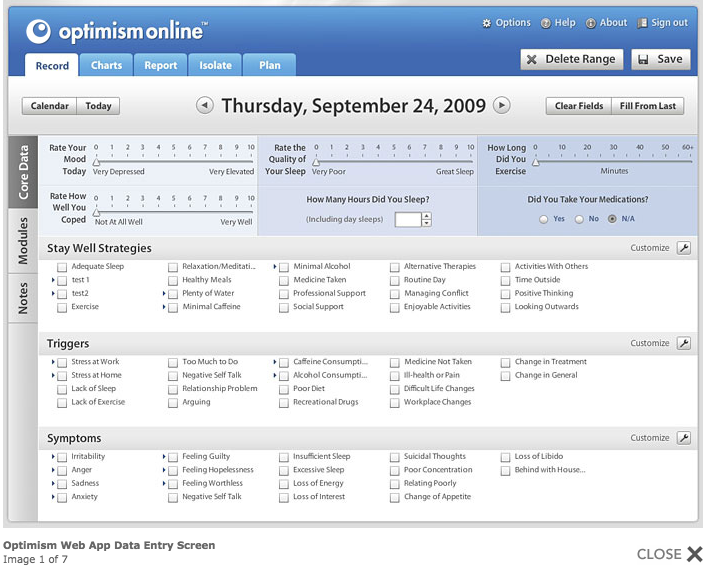
\includegraphics[width=.5\textwidth]{i/optimism1.png}\hfill
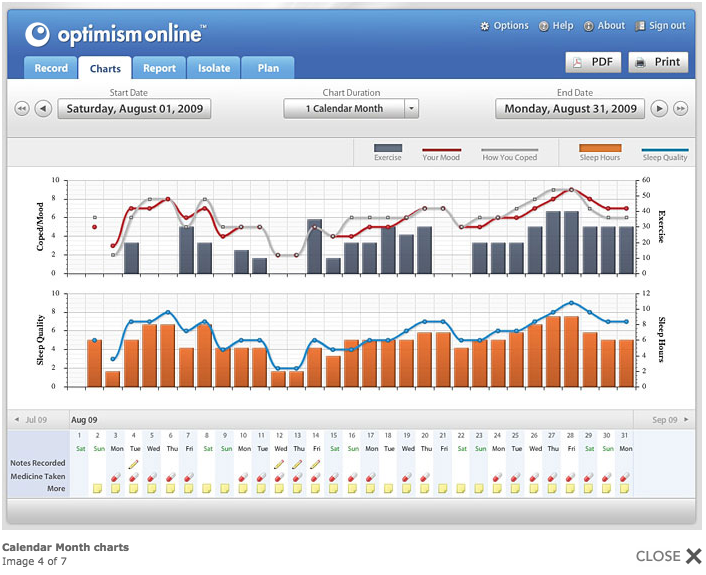
\includegraphics[width=.5\textwidth]{i/optimism2.png}
\label{fig:optimism}
\end{figure}

While Optimism is similar in it's aims to this project, it is a more \enquote{heavy duty} mental health management app, whereas the proposed system in this project is a more lightweight, general purpose self-management app. Optimism clearly has a significantly higher response burden than the proposed system in this project. It does have a wider array of features, but while this can be a positive in terms of aiding users, it means that users will need to spend time learning how to use and interpret the system.

Also, a key part of the proposed system is making use of data that already exists about a user (via existing application APIs), which is a feature not included in Optimism.

\subsection{Exist} \label{exist}
Exist \parencite{exist} is similar to the proposed application from an API data import context. It also produces visualisations of this data, but with some key differences. It imports API data, then produces a dashboard of correlations rather than allowing the user to build visualisations themselves. While Exist is not designed for health or mental health tracking, it has the potential to be used for this, and is actually very impressive in terms of analysing the correlations in data.

There are various issues with Exist however. The study by \citeauthor{jones2016sensemaking} (\citeyear{jones2016sensemaking}) that investigated challenges in sensemaking, was in fact carried out using Exist. The various pre-built visualisations, as well as lack of customisation, can result in users not being able to interpret their data effectively.

\subsection{Zenobase}
Zenobase \parencite{zenobase} is similar to the proposed system from both an API data import and visualisation building context. Zenobase allows users to \enquote{store, aggregate and visualize your data}. It again imports API data, but unlike Exist allows users to build custom visualisations from this data.

This is similar to the functionality of the proposed system. A feature of note that Zenobase has, that is not yet planned for the proposed system, is the ability to manually import data. This means that Zenobase could, while significantly more difficult and time consuming, be used in the exact same way as the proposed system for self-management of mental health and wellbeing.

The system proposed in this project instead has the ability to record a very restricted amount of user data through the SWEMWBS questionnaire. While this simplicity is an advantage of the proposed system, allowing users to also manually import of data would be a nice addition. This may have to be identified as future work.

Zenobase seems to be extremely flexible, and allows the user to interrogate their data in a large number of ways. As a side effect of this, it is quite complex to use and understand. Having tested the system, this does not seem to be due to the design, but due to the flexibility and large number of ways that Zenobase allows users to visualise their data.

This flexibility is clearly an advantage for those users that want it, and the proposed project would not hope to compete with Zenobase in this respect. However, the higher difficulty and complexity may not be accepted by all users, especially those that are not as serious about interrogating their data.

\subsection{Fluxstream}
Like Zenobase, Fluxstream \parencite{fluxstream} also allows users to provide API credentials (via \enquote{connectors}), import their data, and build visualisations from this imported data.

Fluxstream consists of two core applications: a Calendar app and a BodyTrack app. The first of these divides visualisations into various \enquote{tabs}, such as a clock, dashboards, a map and a timeline. This seems to encounter the same challenge as exist: too many options of data interpretation are being provided simultaneously.

It does seem to be very powerful in collating data. The timeline feature for example can be used to map the data from lots of \enquote{connectors}, allowing the user to view all of their activity in one \enquote{feed}. However, the complexity of comprehending the data may deter some users.

The BodyTrack app includes a \enquote{grapher}, allowing the user to build custom visualisations.

\newpage
An image of this can be seen in Figure \ref{fig:fluxstream} (image taken from video on \parencite{fluxstream}):
\begin{figure}[ht]
\centering
\caption{Fluxstream BodyTrack Grapher}
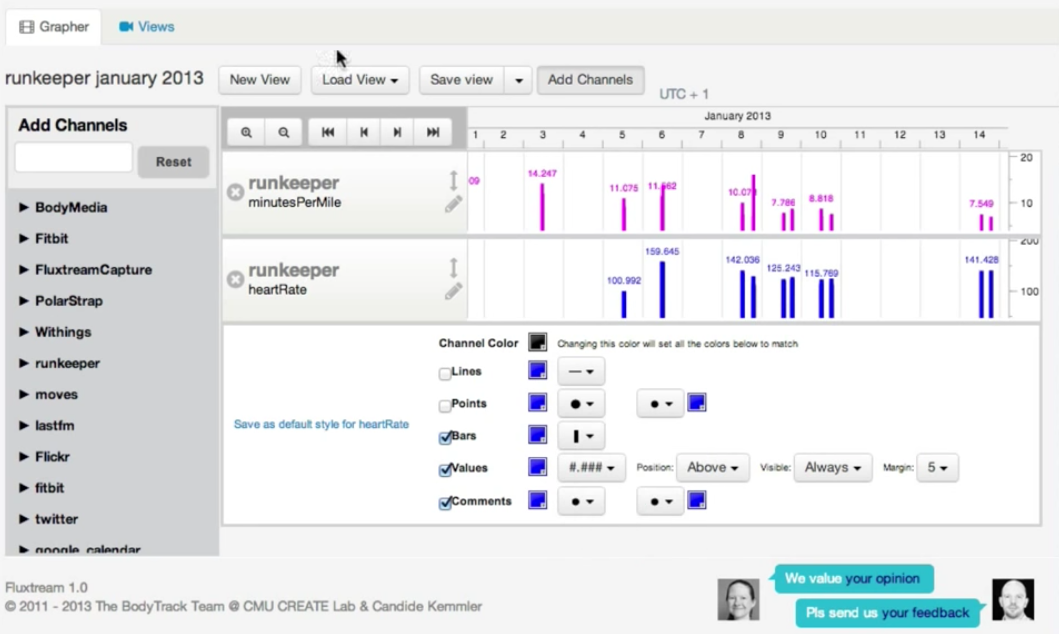
\includegraphics[width=\textwidth]{i/fluxstream.png}
\label{fig:fluxstream}
\end{figure}

This again seems very flexible, but also complicated and very difficult to use, which could again turn users away from the system.

Another issue is that there doesn't seem to be a way to record or import data manually into Fluxstream. Also, Fluxstream does not currently support any mental health and wellbeing tracking apps. This means that it may be impossible, or at least very difficult, for users to use Fluxstream as a mental health tracking/self management tool.

\subsection{Summary}
The four systems reviewed in this section were similar to the proposed system in different ways. Reviewing these existing systems provided some extremely useful insight on how the proposed project can differentiate itself from similar systems. A summary of these insights is provided below:
\begin{itemize}
\item The system will combine user submitted mental health and wellbeing data with API data.
  \begin{itemize}
  \item None of the systems reviewed do this explicitly.
  \item Optimism allows user submitted mental health data, but no API data.
  \item The other three apps allow importing of API data, but no mental health data.
  \item The closest to allowing this is Zenobase, which allows manual data importing. This however would be harder and more time consuming for the user, and would require them to develop their own way of measuring their wellbeing.
  \end{itemize}
\item The system will include a \emph{simple} visualisation building tool.
  \begin{itemize}
  \item Exist and Optimism generated (fairly) fixed visualisations.
  \item Zenobase and Fluxstream included very flexible, complex and difficult to use visualisation building and customisation tools.
  \item The proposed system could, when compared to Zenobase and Fluxstream, sacrifice flexibility to make the system easier to use and understand.
  \end{itemize}
\end{itemize}

\chapter{Requirements Specification}
\section{Introduction}
This chapter will detail the functional and non functional requirements for the various areas of the system. These requirements were obtained and developed primarily from existing research in the area, as discussed in detail in section \ref{litsurvey}, as well as from personal experience and desires for the project. They will encompass the results of the literature survey, and the aims and objectives discussed in sections \ref{aims} and \ref{objectives} respectively. Most of the requirements are unambiguous and intuitive, based on the sources just discussed. However, where a requirement seemed vague and/or its origins seemed to be unclear, an additional sentence or two has been included to justify the requirement, and explain both where it came from and why it is necessary.

Many projects develop requirements from user interviews and surveys, but this wasn't done for this project for various reasons. Firstly, this is an academic project, so is better suited to requirements based on existing literature. Secondly, a goal of this system was to provide a proof of concept that can be built on in the future, rather than a full working system. It may be  advantageous in the development of requirements for future work to consult potential users from the various user groups. There are many possible users, such as those who do not suffer from a diagnosed mental health condition, those that are in treatment and those that are post-treatment. The opinions of all of these may be useful for future work and improvements to the system, but for this project only academic research, personal experience and desires for the project were considered, in order to limit the scope of the project and produce an extensible system for future research and development.

\section{Requirements Structure and Terminology}
\subsection{Structure}
This project consisted of the development of three separate software systems: a mobile app, a web app and an \enquote{application programming interface} (API). These separate software systems were intentionally designed to be entirely separate from one another, as will be discussed further in chapter \ref{chap:design}. This is important to mention here because, as a result of this, the requirements are divided into three separate sections; one for each of the separate software systems. Each of these sections is then divided into functional and non-functional requirements, where functional requirements describe \enquote{what the system does}, and non-functional requirements describe \enquote{how the system works}.

\subsection{Prioritisation Terminology}
These requirements use the \enquote{MoSCoW} method for prioritisation \parencite{moscowmethod}. This is a technique that consists of the terminology seen in table \ref{table:moscow} (term descriptions derived from \parencite{moscowmethod}).

\begin{table}[ht]
\centering
\caption{MoSCoW Method for Requirements Prioritisation Terminology}
\label{table:moscow}
\begin{tabular}{|p{4cm}|p{10cm}|}
\hline
\textbf{Term} & \textbf{Description} \\ \hline
Must have & These are needed for the \textbf{M}inimum \textbf{U}sable \textbf{S}ubse\textbf{t} (\textbf{MUST}) of requirements. That is, they are absolutely required for the system to be viable. Without them, the system does not fulfil a primary goal, provides no value, or is unsafe in some way. \\  \hline
Should have & These are important but not absolutely vital. If they are not completed, some workaround may be possible. The system will still be viable and usable, but may be inefficient or awkward to use. \\ \hline
Could have & These are desirable but not as important as \enquote{should have} requirements. They very much depend on time constraints, and can often be dropped if deadlines are approaching. Although they improve the system, they are not really necessary for the system to be viable. \\ \hline
Won't have this time & These are explicitly defined as requirements that will not be met by the system in this release. Explicitly defining these is useful for limiting the scope of a project/release, as it prevents ambiguity and these requirements from being introduced as extra work at a later date. \\ \hline
\end{tabular}
\end{table}

This project is of course, like many projects, time limited. This method of prioritisation was extremely useful in defining and limiting scope, and in deciding which functionality should be implemented first, and what could be dropped should problems occur and/or time constraints apply.

\subsection{Further Terminology}
The requirements also refer to \enquote{major} and \enquote{minor} bugs. These are defined in table \ref{table:bugsterminology}.
\begin{table}[ht]
\centering
\caption{Major and Minor Bugs Terminology}
\label{table:bugsterminology}
\begin{tabular}{|p{4cm}|p{10cm}|}
\hline
\textbf{Bug} & \textbf{Description} \\ \hline
Major & These cause the system to not meet the requirement in question, or meet the requirement but significantly impact the system in some other way, such as security issues, or major user experience issues. For example, if information shifts \enquote{off-screen}, and so is invisible to the user, this is a fairly major user experience issue. \\  \hline
Minor & These are unintended, but the system still meets the requirement in question, and the consequences are not particularly severe. For example, if content shifts and makes information difficult to read, or simply makes the software look unprofessional. This is undesirable, but still a fairly minor issue, so would be classed as a minor bug.\\ \hline
\end{tabular}
\end{table}

\section{Requirements} \label{reqs}
\subsection{Mobile App}
The mobile app is intended to be very small and simple. It is not a mobile version of the web app, but is instead a simple piece of software to allow users to record their wellbeing quickly using their phone (and hence carry out ecological momentary assessment, as discussed in section \ref{sec:ema}). For this reason, there are a fair amount of \enquote{won't} requirements, so as to keep the software simple and limit the scope. That being said, the requirements for the mobile app are as follows:

\subsubsection{Functional}
\begin{enumerate}
\item Must allow the user to log in.
\item Must allow the user to log out.
\item Should allow the user to create an account.
\item Must allow the user to record their wellbeing.
  \begin{enumerate}
  \item Must have a SWEMWBS questionnaire (see section \ref{swemwbssection}).
  \item Must submit total score of SWEMWBS questionnaire.
  \end{enumerate}
  \item Must submit date and time with wellbeing score.
\item Could have a recent wellbeings table, displaying user's recent wellbeing recordings.
\item Should encourage user to visit the web app to connect existing apps and analyse their wellbeing data.
\item Won't have ability to manage user account.
  \begin{enumerate}
  \item Won't have ability to change user email.
  \item Won't have ability to change user password.
  \item Won't have ability to recover password.
  \end{enumerate}
\item Won't have ability to connect existing apps.
\item Won't have ability to produce and view visualisations.
\end{enumerate}

\subsubsection{Non-functional}
\begin{enumerate}
\item Should allow users to access the SWEMWBS questionnaire within 4 'taps' (email, password, log in, record). Note this of course does not include typing of email and password.
\item Must be built using \enquote{React Native} \parencite{reactnative} \parencite{reactnativegit} to maximise cross-platform code reuse between iPhone and Android.
\item Should include documentation for developers on how to set up the project and get it running.
\item Must be tested manually on iOS (iPhone), including testing by volunteer testers.
  \begin{enumerate}
  \item Must reveal no major bugs when testing all \enquote{must} requirements.
  \item Should reveal no minor bugs when testing all \enquote{must} requirements.
  \item Should reveal no major bugs when testing all \enquote{should} requirements.
  \item Could reveal no minor bugs when testing all \enquote{should} requirements.
  \item Should reveal no major bugs when testing all \enquote{could} requirements, if these features are implemented.
  \item Could reveal no minor bugs when testing all \enquote{could} requirements, if these features are implemented.
  \item Should also be tested (by volunteer testers) with the goal of identifying missing features, bugs not relating to defined requirements, and usability issues.
  \end{enumerate}
\item Could be effective on Android due to the software being built using React Native.
  \begin{enumerate}
  \item Won't be tested manually on Android.
  \end{enumerate}
\end{enumerate}

\subsection{Web App}
The web app is significantly larger, and incorporates most of the major contributing features of this project, including connecting existing apps and building and viewing visualisations. The web app does almost everything, if not everything the mobile app does, and more. Also note that security is not discussed here, as all data is accessed via the API, so security is a requirement of the API, not the web app.

\subsubsection{Functional}
\begin{enumerate}
\item Must allow the user to log in.
\item Must allow the user to log out.
\item Must allow the user to create an account.
\item Must allow the user to record their wellbeing.
  \begin{enumerate}
  \item Must have a SWEMWBS questionnaire (see section \ref{swemwbssection}).
  \item Must submit total score of SWEMWBS questionnaire.
  \end{enumerate}
\item Must submit date and time with wellbeing score.
\item Should encourage user to download the mobile app to record their wellbeing from their phone.
\item Should allow user to manage user account.
  \begin{enumerate}
  \item Should allow user to change user email.
  \item Should allow user to change user password.
  \item Could allow user to recover password.
  \item Could allow user to verify their email.
  \end{enumerate}
\item Must keep user logged in throughout navigation of application.
\item Should keep user logged in after full page refreshes.
\item Must allow user to connect their Twitter account.
  \begin{enumerate}
  \item Must store this information for use in subsequent requests to Twitter's API, to fetch user's data.
  \item Must be able to fetch user's tweets.
  \end{enumerate}
\item Must allow user to connect their Strava account.
  \begin{enumerate}
  \item Must store this information for use in subsequent requests to Strava's API, to fetch user's data.
  \item Must be able to fetch user's Strava data.
  \end{enumerate}
\item Won't include connection of any applications other than Twitter and Strava, as these are being included as proofs of concept.
\item Must be able to fetch user's SelfReflect wellbeing data.
\item Must allow user to build visualisations combining these any of three sources of data (SelfReflect wellbeing data, Twitter data and Strava data).
  \begin{enumerate}
  \item Must provide one visualisation built from SelfReflect wellbeing data.
  \item Must provide one visualisation built from Twitter data.
  \item Must provide one visualisation built from Strava data.
  \item Should allow Twitter and Strava data to be directly compared to SelfReflect wellbeing data in some way, via these visualisations.
  \item Could also allow these data sources to be directly compared with one another in some way, via these visualisations.
  \item Won't include interactive visualisations (such as \enquote{zoom}, \enquote{click and drag} etc.).
  \end{enumerate}
\item Should provide a guide/help page for the user, with a \enquote{step-by-step} guide on how to use the system.
\end{enumerate}

\subsubsection{Non-functional}
\begin{enumerate}
\item Must be built using React \parencite{react} and Redux \parencite{redux}, meaning it is built entirely in JavaScript.
\item Should be a \enquote{one page} application. That is, built using AJAX (asynchronous JavaScript and XML) requests only. This means there will be no full page requests after the initial request. This is what allows separation of functional requirements 8 and 9.
\item Should use ReactD3 to build visualisations, which is an open source library for building charts using React \parencite{reactd3}.
\item Should incorporate and be styled using Skeleton CSS, which is a \enquote{dead simple, responsive boilerplate} \parencite{skeletoncss}.
\item Could be responsive due to the use of Skeleton CSS. That is, the application will adjust styling and work on various screen sizes. Note this is easily tested by simply resizing browser windows. Hence:
  \begin{enumerate}
  \item Could work on mobile phones.
  \item Could work on tablets.
  \item Should be tested on various browser window sizes to test responsiveness, with regard to each requirement.
  \end{enumerate}
\item Should run in three major modern internet browsers.
  \begin{enumerate}
  \item Must run in Google Chrome.
  \item Should run in Safari.
  \item Should run in Firefox.
  \end{enumerate}
\item Should include documentation for developers on how to set up the project and get it running.
\item Must be tested manually, including testing by volunteer testers.
  \begin{enumerate}
  \item Must reveal no major bugs when testing all \enquote{must} requirements.
  \item Should reveal no minor bugs when testing all \enquote{must} requirements.
  \item Should reveal no major bugs when testing all \enquote{should} requirements.
  \item Could reveal no minor bugs when testing all \enquote{should} requirements.
  \item Should reveal no major bugs when testing all \enquote{could} requirements, if these features are implemented.
  \item Could reveal no minor bugs when testing all \enquote{could} requirements, if these features are implemented.
  \item Should also be tested (by volunteer testers) with the goal of identifying missing features, bugs not relating to defined requirements, and usability issues.
  \end{enumerate}
\end{enumerate}

\subsection{API}
The API is the server; it is where storage and retrieval of all user data happens. It is a huge part of the system and is the source of many important features such as user management, wellbeing data storage and retrieval, connection of existing applications, fetching of data from existing applications and security/authentication.

\subsubsection{Functional}
\begin{enumerate}
\item Must allow creation of users.
\item Should allow fetching of users.
\item Should allow update of users.
  \begin{enumerate}
  \item Should allow update of email.
  \item Should allow update of password.
  \item Could allow deletion of users.
  \item Could allow password recovery.
  \item Could allow verification of user email.
  \end{enumerate}
\item Must allow storage of SWEMWBS wellbeing score.
  \begin{enumerate}
  \item Must allow storage of data and time of submission with wellbeing score.
  \item Must include a copy of the SWEMWBS conversion table, as seen in appendix \ref{swemwbsconversiontable}
  \item Must be able to convert raw to metric SWEMWBS score, using this table.
  \end{enumerate}
\item Must allow retrieval of recent SWEMWBS metric wellbeing scores, with date and time.
  \begin{enumerate}
  \item Could allow specification of how many score entries to return.
  \end{enumerate}
\item Must allow connection and storage of Twitter credentials
\item Must allow retrieval of user's recent tweets, if they have connected Twitter. This should be exactly as defined by Twitter's API, and not modified in any way.
\item Must allow connection and storage of Strava credentials.
\item Must allow retrieval of user's recent Strava data, if they have connected Twitter. This should be exactly as defined by Strava's API, and not modified in any way.
\item Won't include connection of any applications other than Twitter and Strava, as these are being included as proofs of concept.
\item Must accept and return data as JSON (JavaScript Object Notation).
\item Must require authentication for any request that returns a user's data.
  \begin{enumerate}
  \item Must allow user to provide a valid email and password in exchange for an authentication access token.
  \item Must require a valid token to access user's data (i.e. all requests other than requests to create a user, or requests for a token).
  \item Could allow refreshing of tokens before they expire.
  \item Must prevent user's from accessing other user's data, or any other restricted data, regardless of access token.
  \end{enumerate}
\end{enumerate}

\subsubsection{Non-functional}
\begin{enumerate}
\item Must be built using Node.js (a JavaScript runtime for writing server side JavaScript code) \parencite{nodejs} and Express (a \enquote{fast, unopinionated, minimalist web framework for Node.js}) \parencite{expressjs}. These are modern tools that will both speed up development and likely produce faster, more reliable, higher quality code. Node.js is very popular and, as a result, there exists lots of compatible open source software compatible that this project can take advantage of.
\item Must use MySQL for database access (the \enquote{world's most popular open source database}) \parencite{mysql}. There is little reason to use anything else for database access for this project, as MySQL is suited for all the project's needs. There are alternatives, but for the purposes of this project, these would not provide any significant benefits over MySQL.
\item Must store passwords in a secure, hashed format. This is so that, even if this database is somehow accessed, user's passwords will not be lost.
\item Should be a RESTful API. REST is Representational State Transfer and employs a stateless architecture where each request is independent. This is a modern standard and best practise for building APIs. This stateless architecture means each request must be authenticated individually. Endpoints are implemented as resources such as /User and are accessed using http \enquote{verbs} (GET, PUT, PATCH, POST, DELETE) \parencite{httpmethods}.
\item Must include extensive documentation.
  \begin{enumerate}
  \item Must include documentation for developers on how to set up the project and get it running.
  \item Must have documentation for all endpoints. This is absolutely essential to make the API professional and, more importantly, to make the entire SelfReflect system extensible. Developers must understand the API, be able to use the API, and be able to extend the API if this project is to be built upon in the future.
  \end{enumerate}
\item Should have automated tests. This section of the project deals with user data and security, so correct and reliable behaviour is essential. Also, while the API can be manually tested indirectly via the web and mobile apps, it cannot be manually tested directly, so automated tests are important.
  \begin{enumerate}
  \item Should have automated tests covering at least 70\% of lines of code.
  \item Could have automated tests covering at least 95\% of lines of code.
  \end{enumerate}
\end{enumerate}

\chapter{Design} \label{chap:design}
This chapter will detail the design of both the system as a whole, and the three separate parts of the system (mobile app, web app and API), with regard to the requirements specified in section \ref{reqs}. Functional and non-functional requirements from this point onwards will be referred to as \enquote{F} and \enquote{NF} requirements respectively. Requirements referenced in each section will always refer to the corresponding section in section \ref{reqs}, unless explicitly stated.

\section{Overall System}
Many modern software systems are designed using a client-server architecture. That is, one server and many clients, such as for web pages. Additionally, many successful applications have external APIs, which allows developers of external applications to build their own interfaces to the data, accessed via the corresponding API. These are the same APIs this project will take advantage of, in order to fetch user data from existing applications, such as Twitter and Strava.

The system developed in this project will take a similar approach to this client-server, API based design. Most systems developed using these methods include internally developed client applications, that access the data differently from externally developed applications. The system in this project however will not do this. The mobile and web apps will access the data entirely via the API, and as such will essentially be no different to applications developed externally by other developers, as shown in Figure \ref{fig:OverallSystem}. This encourages, and to an extent guarantees, maximum extensibility for the project. The internally developed client applications will have the same access to the data as externally developed applications, meaning there is no disparity between the abilities of internally and externally developed client applications.

\begin{figure}[ht]
\centering
\caption{Overall System Architecture}
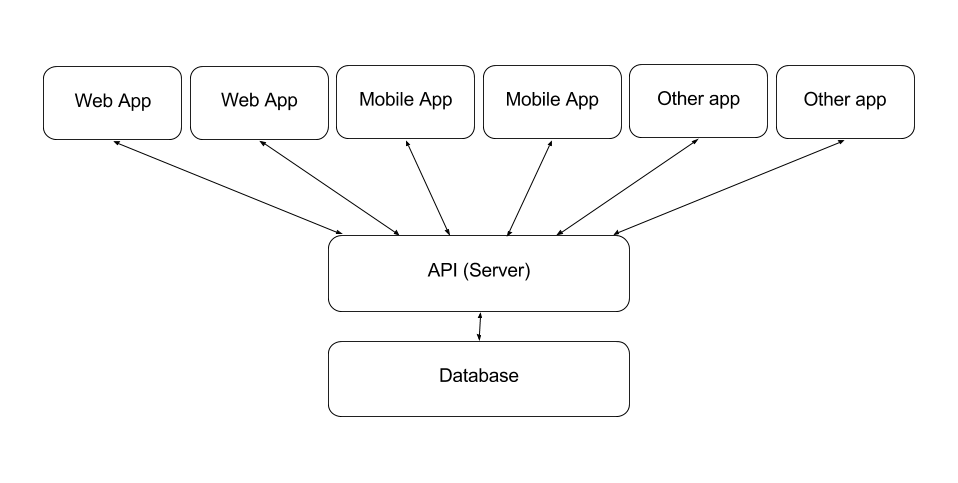
\includegraphics[width=\textwidth]{i/OverallSystem.png}
\label{fig:OverallSystem}
\end{figure}

\newpage
\section{Mobile App}
One internal client application that will communicate via the API is the SelfReflect mobile app. This is a fairly simple application, with the primary goal of allowing the user to record their mental health and wellbeing easily via a mobile app, in order to facilitate ecological momentary assessment.

This application will be built in \enquote{React Native} \parencite{reactnative}. React Native is a framework for building native mobile apps using JavaScript. It uses the same native components as are used when developing in Objective-C or Java (for iOS and Android respectively), but uses JavaScript to assemble them. A huge advantage of this is that almost all code, if not all code, is cross-platform. This is the reason for NF2, NF4 and NF5. Although the mobile app will only be tested on iOS, it may well be as (or almost as) effective on Android, purely by virtue of the technologies used to build it.

To facilitate the design of the mobile app, various \enquote{wireframes} were created to provide some plan as to how the application should look. These are low fidelity prototypes, and images of each will be included and referenced throughout this section.

\subsection{Login and Register}
The first page the user sees after opening the mobile app will be a simple login screen, with email and password fields, and two buttons: one to login, and one to navigate to a register screen. The wireframe for this screen can be seen in Figure \ref{fig:mobilelogin}.

\begin{figure}[ht]
\centering
\caption{Mobile App Login Screen Wireframe}
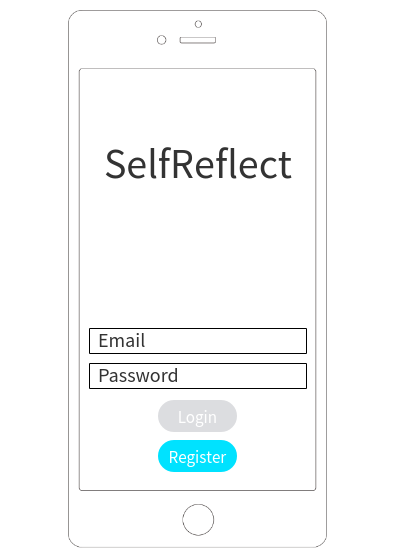
\includegraphics[width=0.3\textwidth]{i/mobilelogin.png}
\label{fig:mobilelogin}
\end{figure}

The user can then either log in, satisfying F1, or navigate to the register screen, satisfying F3. The wireframe for the register screen can be seen in Figure \ref{fig:mobileregister}.

\begin{figure}[ht]
\centering
\caption{Mobile App Register Screen Wireframe}
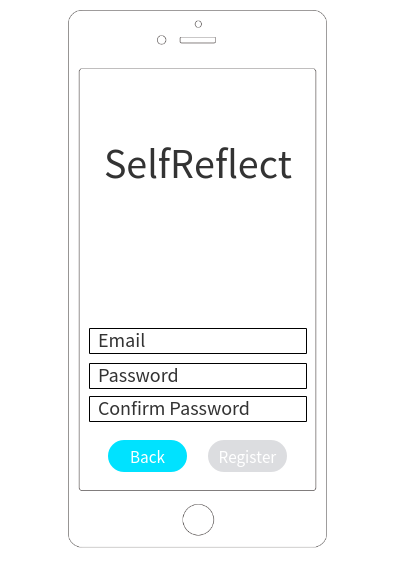
\includegraphics[width=0.3\textwidth]{i/mobileregister.png}
\label{fig:mobileregister}
\end{figure}

Both logging in and registering will then need to communicate with the SelfReflect API, in order to either create the user in the SelfReflect database, or to validate login credentials before allowing the user to log in. The mobile app must therefore be able to handle both successful and erroneous responses from the API (such as invalid password, email already exists, server error etc.), and give the user some feedback on these.

A successful login will result in the API responding with an access token (see section \ref{sec:apiauth}). This will then have to be stored locally in the mobile app's state, so that it can be sent with subsequent requests, as discussed in the following sections.

\subsection{Home Page}
After logging in successfully, the user will be taken to a home page. This page will include:
\begin{enumerate}
\item A table of recent recordings, satisfying F6. Note this is a \enquote{could} requirement, so may be dropped if time constraints apply.
\item A message to encourage the user to visit the SelfReflect web app, satisfying F7.
\item A button to navigate to a SWEMWBS questionnaire, to record wellbeing.
\end{enumerate}

Also note that all pages (once logged in), will contain a button at the top of the page to log out of the app, satisfying F2. The wireframe for this home page can be seen in Figure \ref{fig:mobilehome}.

\begin{figure}[ht]
\centering
\caption{Mobile App Home Screen Wireframe}
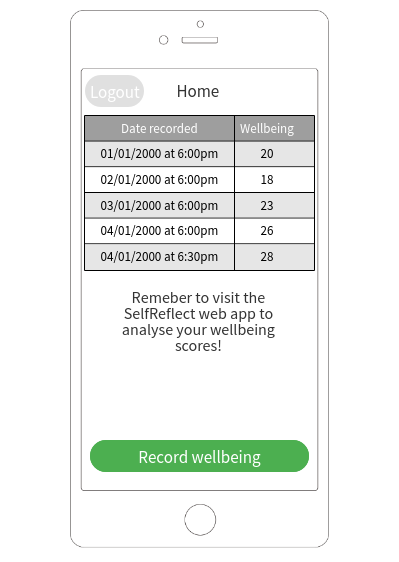
\includegraphics[width=0.3\textwidth]{i/mobilehome.png}
\label{fig:mobilehome}
\end{figure}

The table of recent recordings on this screen is, of course, dynamically generated as it is fetched from the API. As discussed earlier, this will require the mobile app to make a request to the API, using the access token obtained from the user logging in. The API will then respond with the user's recent recordings, and the table can be generated.

Also, the button to record wellbeing satisfies NF1, as it allows users to get to the SWEMWBS questionnaire in 4 taps. These are: tap email (then input), tap password (then input), tap login, tap record button.

\subsection{SWEMWBS Questions}
If the user taps the \enquote{record wellbeing} button, they will navigate to the SWEMWBS questions, satisfying F4.1. As mobile screens are small, the questions will be presented to the user one at a time. All of these question screens will be similar, so only one wireframe was created, as can be seen in Figure \ref{fig:mobilequestion}. In this wireframe, \enquote{often} has been selected as an answer, hence the green background.

\begin{figure}[ht]
\centering
\caption{Mobile App SWEMWBS Question Screen Wireframe}
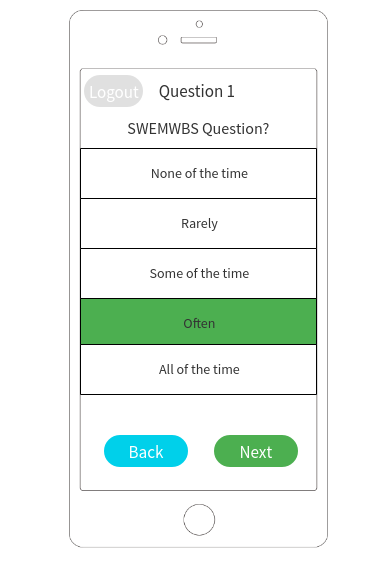
\includegraphics[width=0.3\textwidth]{i/mobilequestion.png}
\label{fig:mobilequestion}
\end{figure}

The only small difference between different question screens is that the last question screen will contain a \enquote{submit} button, rather than a \enquote{next} button. Note that all questions are mandatory; the next buttons (and the submit button) will all be disabled until the question on that page has been answered.

The submit button will sum the answers to all the questions and submit these via the SelfReflect API, satisfying F4.2. It will also compute the date and time of submission, and submit this alongside the computed wellbeing score, satisfying F5. It is important to compute this \enquote{client-side} rather than \enquote{server-side}, as this is (to the user) when the wellbeing was recorded. If this was computed server-side and some delay happened, the user could end up with a wellbeing recorded at a time significantly different from when they actually tapped submit. Computing this client-side makes this almost impossible, as long as date and time are computed and communicated correctly.

\section{Web App}
The second, larger internal client application that will communicate via the API is the SelfReflect web app. This is much more complex and has many more features than the mobile app. It allows everything the mobile app allows, but also enables the user to connect existing apps and produce visualisations from their data, fetched from both the SelfReflect API and other connected existing apps (Twitter and Strava).

\section{API and Database}
\subsection{API}
\subsubsection{Authentication} \label{sec:apiauth}

\subsection{Database}
a

\chapter{Implementation}
\section{Mobile App}
a

\section{Web App}
a

\section{API}
\subsection{API}
a

\subsection{Database}
a

\chapter{Testing}

\ldots


\chapter{Results and Discussion}

\ldots


\chapter{Conclusions and Future Work}

\ldots

\printbibliography

\begin{appendices}
\section{SWEMWBS conversion table} \label{SWEMWBS conversion table}
\begin{figure}[ht]
  \centering
  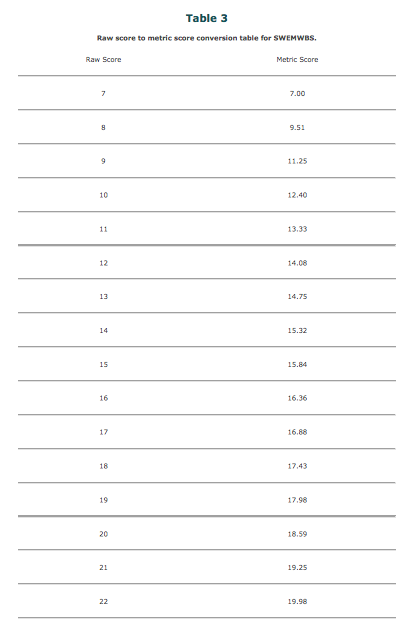
\includegraphics[width =.7\textwidth]{i/swemwbsconversiontable1.png}
  \label{swemwbsconversiontable}
\end{figure}

\begin{figure}[ht]
  \centering
  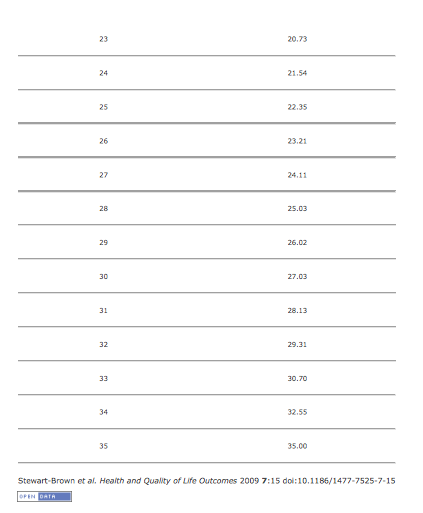
\includegraphics[width =.7\textwidth]{i/swemwbsconversiontable2.png}
\end{figure}
\end{appendices}

\end{document}
